\section{Data analysis and interpretation}

\subsection{Participants}

The sample initially consisted of 61 fictional under-graduate students from a University in Perth, Western Australia who responded to a survey regarding their Facebook use. 

Out of the 61 observations, five were excluded from the dataset with NA responses, and three observations were excluded with responses to the questionnaire as ``0'' (zero). The dataset was then screened for outliers, excluding two observations with reported Facebook logins greater than 50 per week. One observation was excluded, with reported hours spent on Facebook greater than 50 per week. Finally, two observations were excluded, with reported number of close friends greater than 70.

This resulted in a final sample of 48 Facebook users, 3 female, 45 male (M = 0.938, SD = 0.2446) between the ages of 17 to 29 (M = 20.6, SD = 3.206543). Gender is coded as 0 = female and 1 = male in the dataset.

\subsection{Survey}

Each participant filled out a survey which consisted of ten sections. The first section included questions about the participants demography, requesting their age and sex. The second section included questions regarding the amount of Facebook use, requesting self-reported estimates on the number of Facebook logins per week, and hours spent per week on Facebook. The third section included questions regarding the participant's social networking and connection, requesting self-reported estimates on how many Facebook friends they have, how many offline close friends they have, and a 5 point Likert-style scale opinion of their own sociability; 1 = strongly disagree, 5 = strongly agree. 

The fourth and final section included personality surveys, measuring extraversion, self-esteem and social anxiety. Extraversion was measured through a personality test of 25 items, the scores of which were converted to an integer value between 1 and 25. A lower value suggests introversion and a higher value suggests extraversion. Self esteem was measured using a Rosenberg self esteem scale survey of 10 items. The scale ranges between 0 to 30, with scores between 15 to 25 considered normal, and scores below 15 suggesting low self esteem. Social anxiety was measured using a Liebowitz Social Anxiety Scale survey of 24 items, with scores between 55 to 65 suggesting moderate social phobia, scores between 65 to 80 suggesting marked social phobia, 80 to 95 suggesting severe social phobia and scores greater than 95 suggesting very severe social phobia.

%\begin{itemize}
%\item Gender: Binary categorical variable
%\item Facebook friends (FB friends): directly related to Thesis Statement 1
%\item Close friends: secondary variable to test Thesis Statement 1
%\item Sociability: secondary variable to test Thesis Statement 1
%\item Facebook hours: directly related to Thesis Statement 2
%\end{itemize}

\subsection{Descriptive statistics}

This research paper aims to explore the relationship between gender and network size, and the relationship between gender and amount of time spent on Facebook. As such, the following measured variables from the survey have been selected for this research:\\

\begin{itemize}
\item \textbf{Gender:} The categorical variable with binary values, 0 = female or 1 = male.
\item \textbf{Facebook Friends (FB friends):} Primary variable related to testing Thesis Statement 1.
\item \textbf{Close Friends:} Secondary variable related to testing Thesis Statement 1, exploring the possibility that gender is also related to number of close friends offline, and may provide further evidence for Thesis Statement 1.
\item \textbf{Sociability:} Secondary variable related to testing Thesis Statement 1, exploring the possibility that gender may also have a correlation with Sociability, and may provide further evidence for Thesis Statement 1.
\item \textbf{Facebook Hours:} Primary variable related to testing Thesis Statement 2.
\end{itemize}

Table 1 provides centrality and variance measures of the selected variables.\\

\begin{table}[H]
\centering
\caption{Measures of centrality and variance}
\begin{tabular}{r|l|l|l|l|l|l|l|l}
Variable      & Min & Max & Mean   & Median & Mode & Std. Dev & Skew   & Kurt      \\ \hline
Gender        & 0   & 1   & 0.9375 & 1      & 1    & 0.2446   & -3.502 & 10.49     \\ \hline
FB Friends    & 33  & 798 & 290.7  & 275    & 242  & 176.001  & 0.796  & 0.048   \\ \hline
Close Friends & 6   & 53  & 21.73  & 19     & 23   & 12.29    & 0.967  & 0.148    \\ \hline
Sociability   & 2   & 5   & 3.667  & 4      & 4    & 0.7532   & -0.563 & -0.009 \\ \hline
\end{tabular}
\end{table}

%As shown in the table above, and in the histograms and q-q plots to follow, all the variables are non-normally distributed. Therefore, non-parametric inferential tests will be used.

%It is worth noting that men greatly outnumber women in this sample set by 15 to 1. Unfortunately, there is not enough female representation in the dataset to provide any meaningful conclusions in the tests to follow.

With Gender coded as 0 = female and 1 = male, the Gender mean of 0.9375 demonstrates that the majority of participants within this dataset are men. Women only represent 3 of the total 48 observations and will pose a recurring limitation throughout this research paper.

%With such a small number of female participants, there is not enough evidence to provide any meaningful conclusions when testing for any correlations between gender and the selected variables.

Facebook Friends exhibits the highest variance about the mean, with a standard deviation of 176.001. A positive skew of 0.796 and high variance is caused by a potential outlier, with a maximum score of 798. The exclusion of this outlier could possibly normalize the variance and skew, however, the score belongs to an observation from a female participant, and the exclusion would result in a dataset with only 2 female participants. Therefore, it was decided that this observation would not be screened, so that the following tests would include as many female participants as possible.

The figures below include histograms and q-q plots to assist in identifying a normal or non-normal distribution.

\subsubsection{Gender}

Figure 1 shows the histogram for Gender. The blue curve overlay demonstrates a non-normal distribution. Only non-parametric tests are applicable for this variable. The histogram also illustrates the disproportionate amount of female participants in this sample set.

%As previously mentioned, men greatly outnumber women in this study, therefore, no meaningful conclusions can be made from the following tests.

\begin{figure}[H]
\centering
\caption{Histogram: Gender}
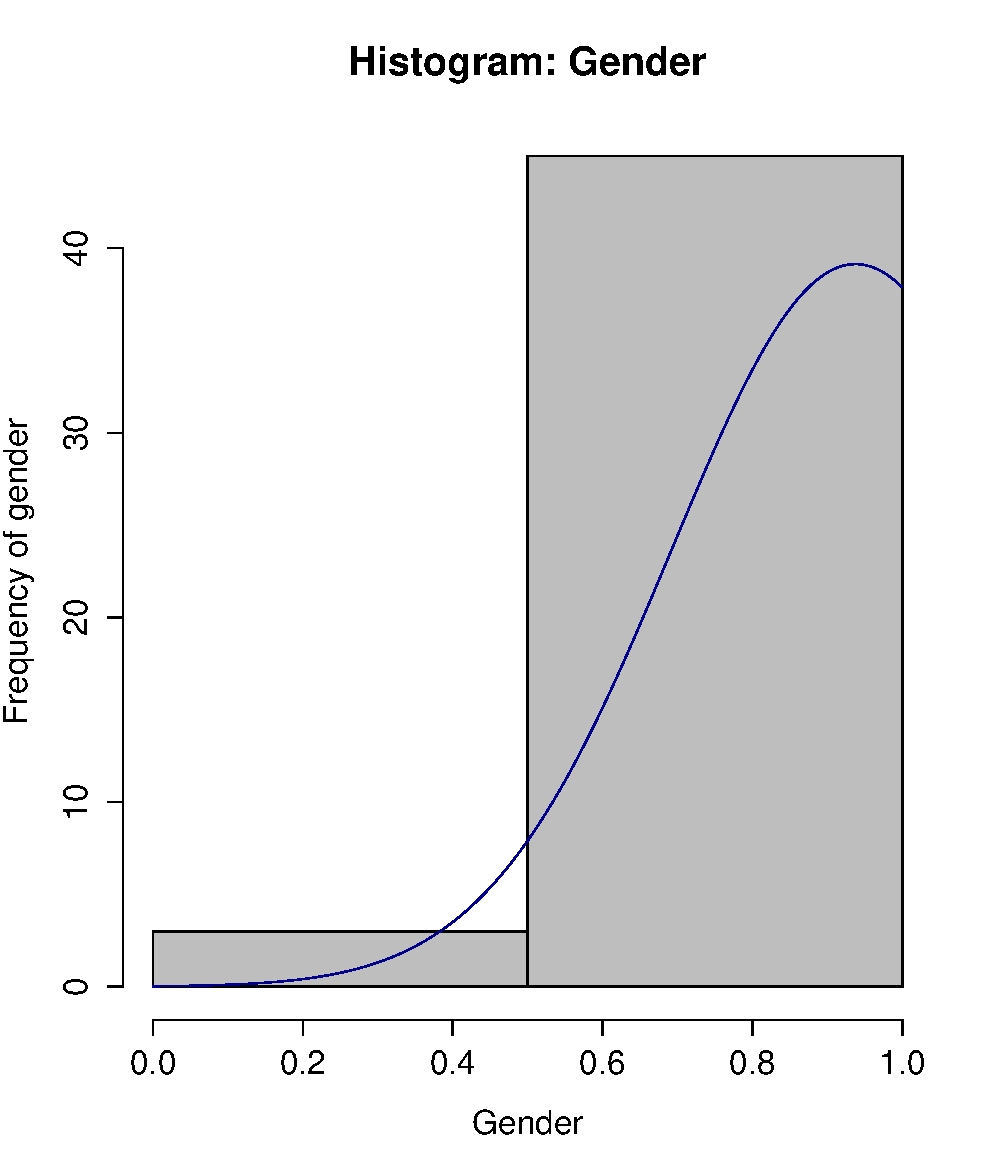
\includegraphics[scale=0.35]{./img/hist_gender.pdf}
\end{figure}

\subsubsection{Facebook Friends}

Figure 2 shows the histogram and normal q-q plot for Facebook Friends. The blue curve overlay on the histogram demonstrates a non-normal distribution. The normal q-q plot also demonstrates a non-normal distribution, as the majority of data-points do not fall on the expected normal distribution line. Only non-parametric tests are applicable for this variable.

\begin{figure}[H]
\caption{Histogram and Normal Q-Q Plot: Facebook Friends}
\centering
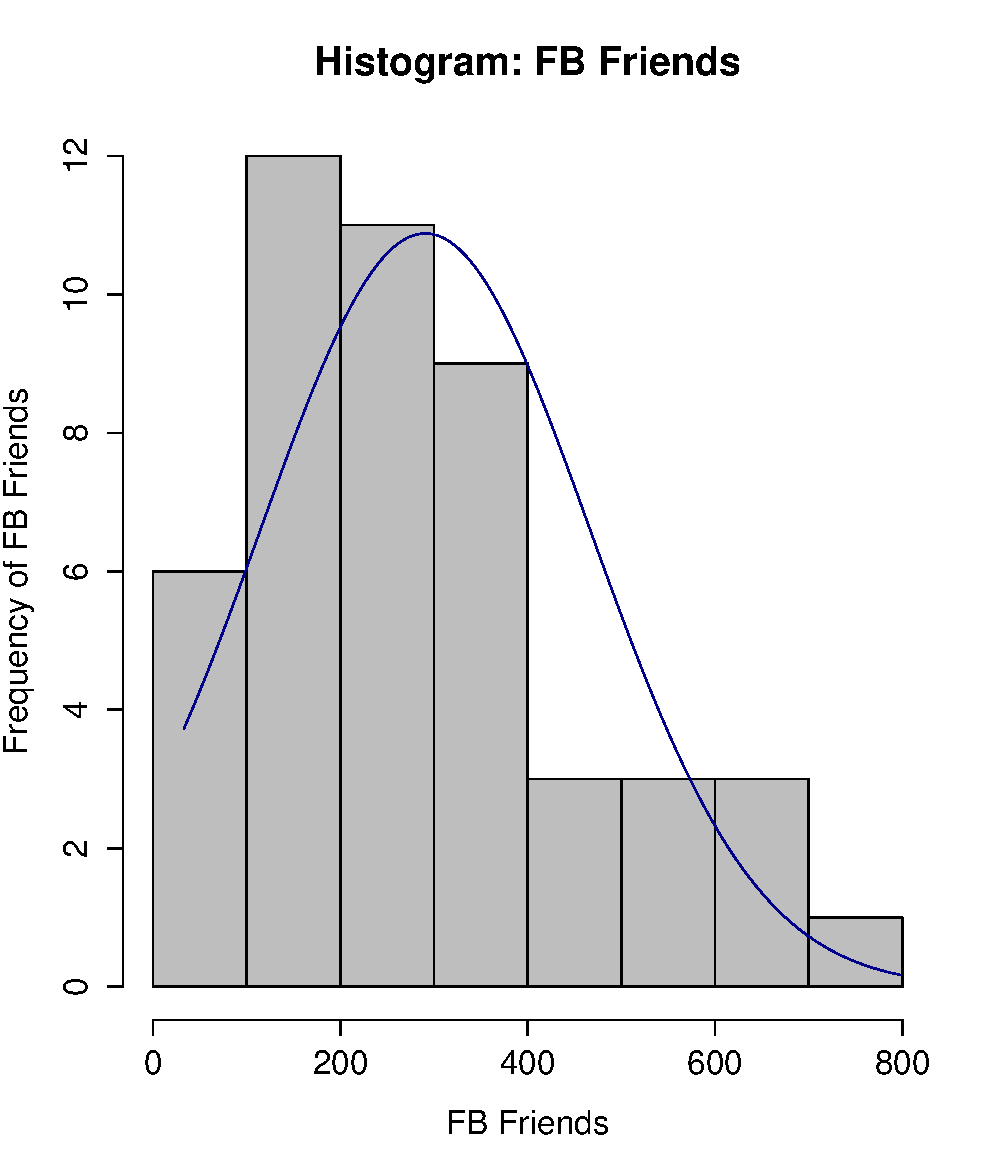
\includegraphics[scale=0.35]{./img/hist_fbfriends.pdf}
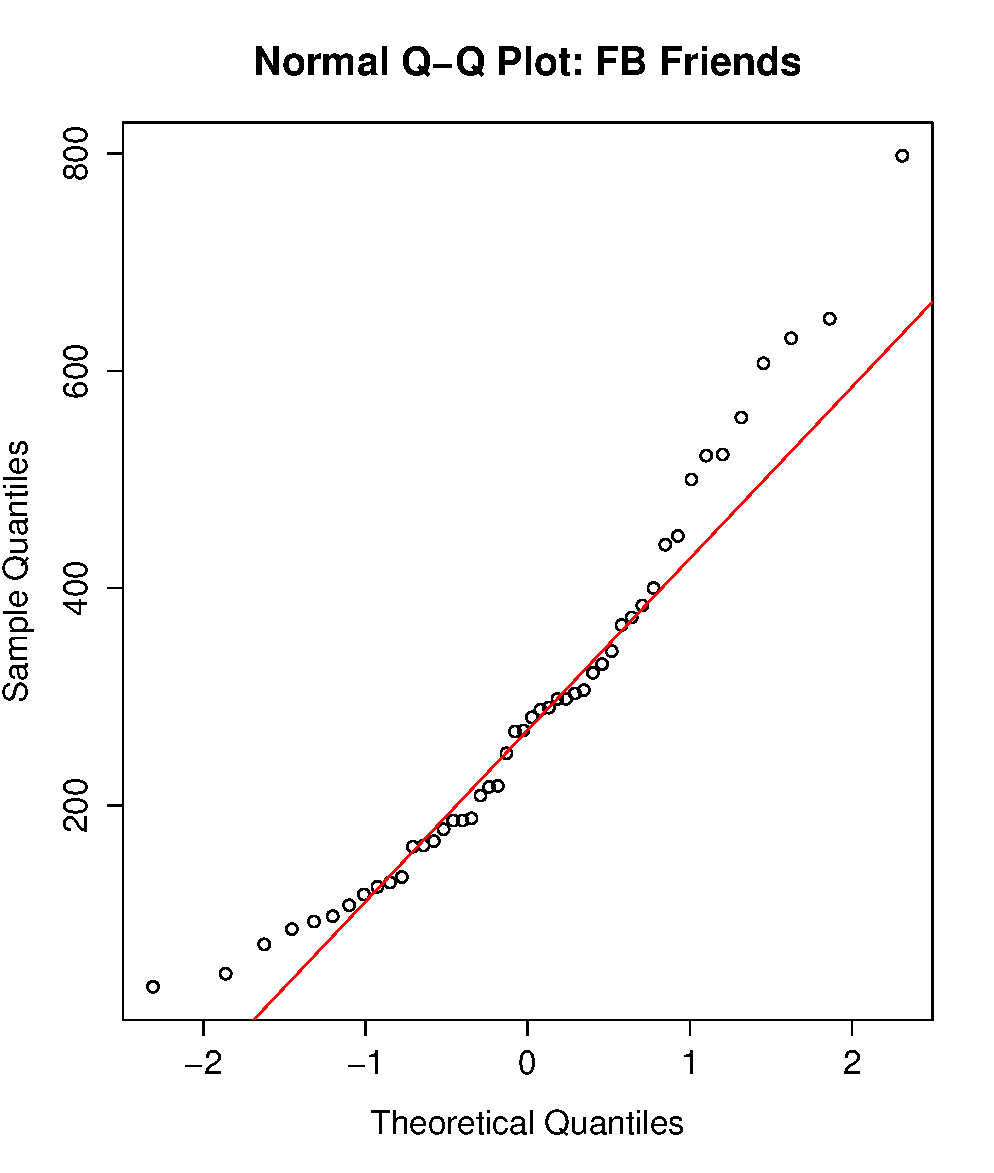
\includegraphics[scale=0.35]{./img/qqplot_fbfriends.pdf}
\end{figure}

\subsubsection{Close Friends}

Figure 3 shows the histogram and normal q-q plot for Close Friends. The blue curve overlay on the histogram demonstrates a non-normal distribution. The normal q-q plot also demonstrates a non-normal distribution, as the majority of data-points do not fall on the expected normal distribution line. Only non-parametric tests are applicable for this variable.

\begin{figure}[H]
\caption{Histogram and Normal Q-Q Plot: Facebook Friends}
\centering
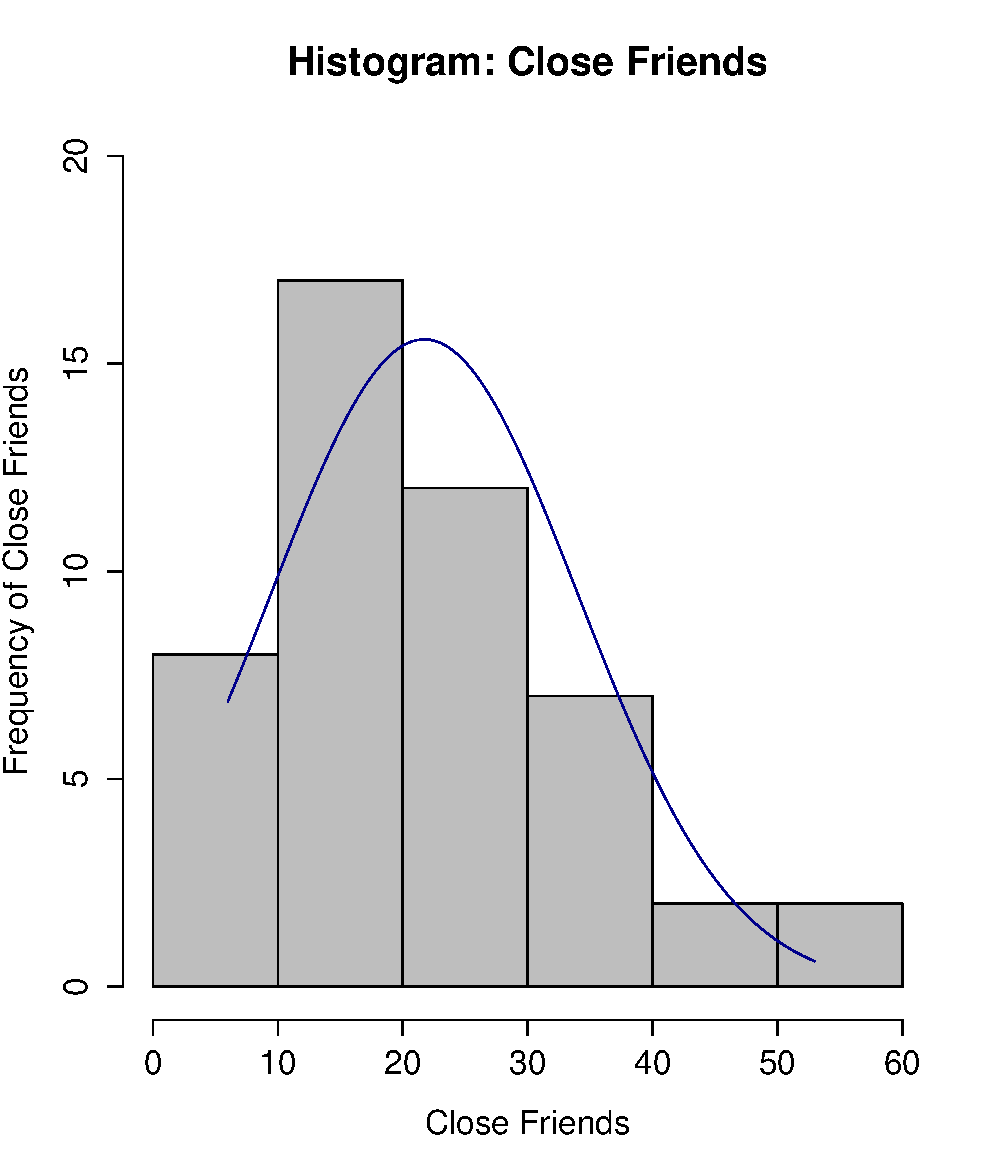
\includegraphics[scale=0.35]{./img/hist_closefriends.pdf}
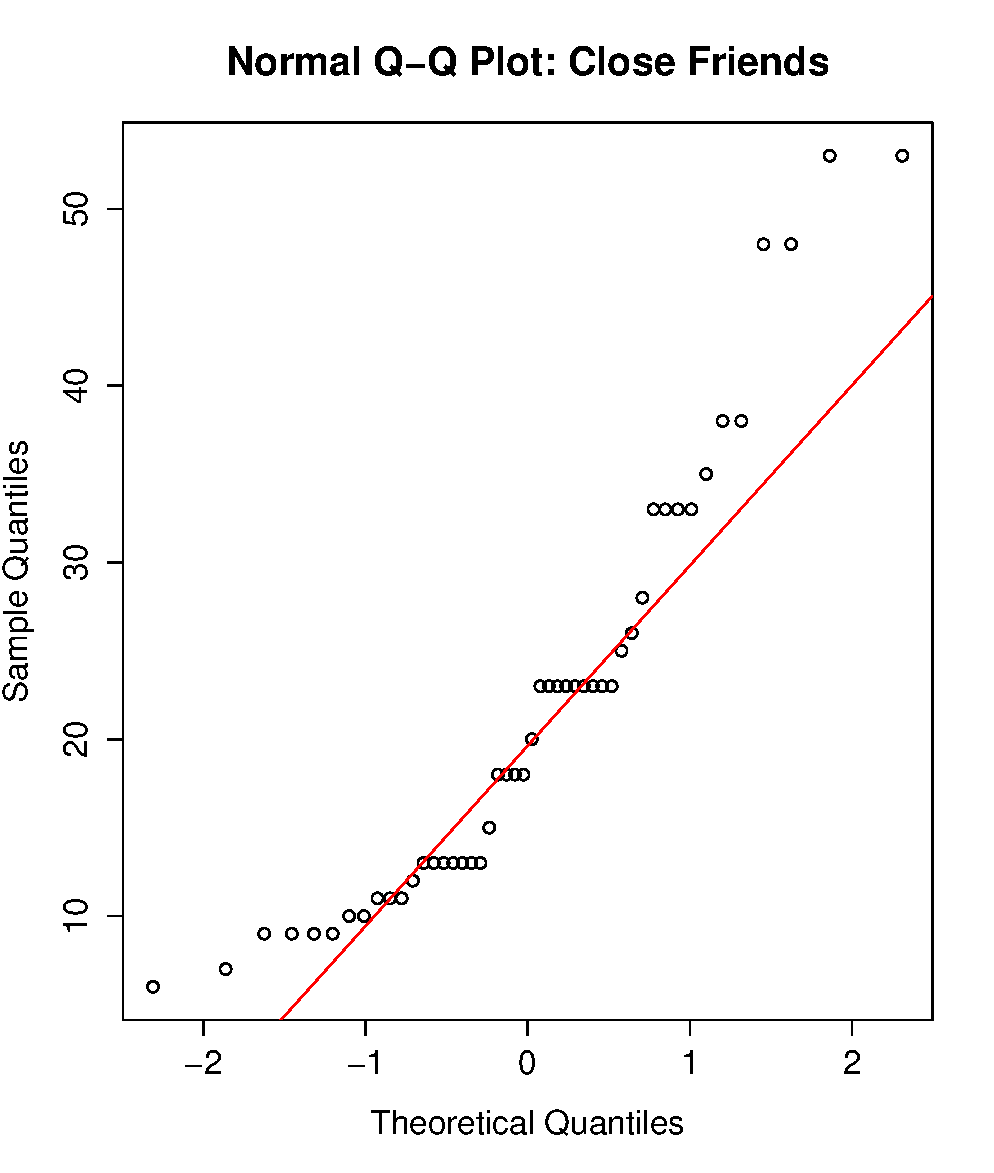
\includegraphics[scale=0.35]{./img/qqplot_closefriends.pdf}
\end{figure}

\subsubsection{Sociability}

Figure 4 shows the histogram and normal q-q plot for Sociability. The blue curve overlay on the histogram demonstrates a non-normal distribution. The normal q-q plot also demonstrates a non-normal distribution, as the majority of data-points do not fall on the expected normal distribution line. Only non-parametric tests are applicable for this variable.

\begin{figure}[H]
\caption{Histogram and Normal Q-Q Plot: Sociability}
\centering
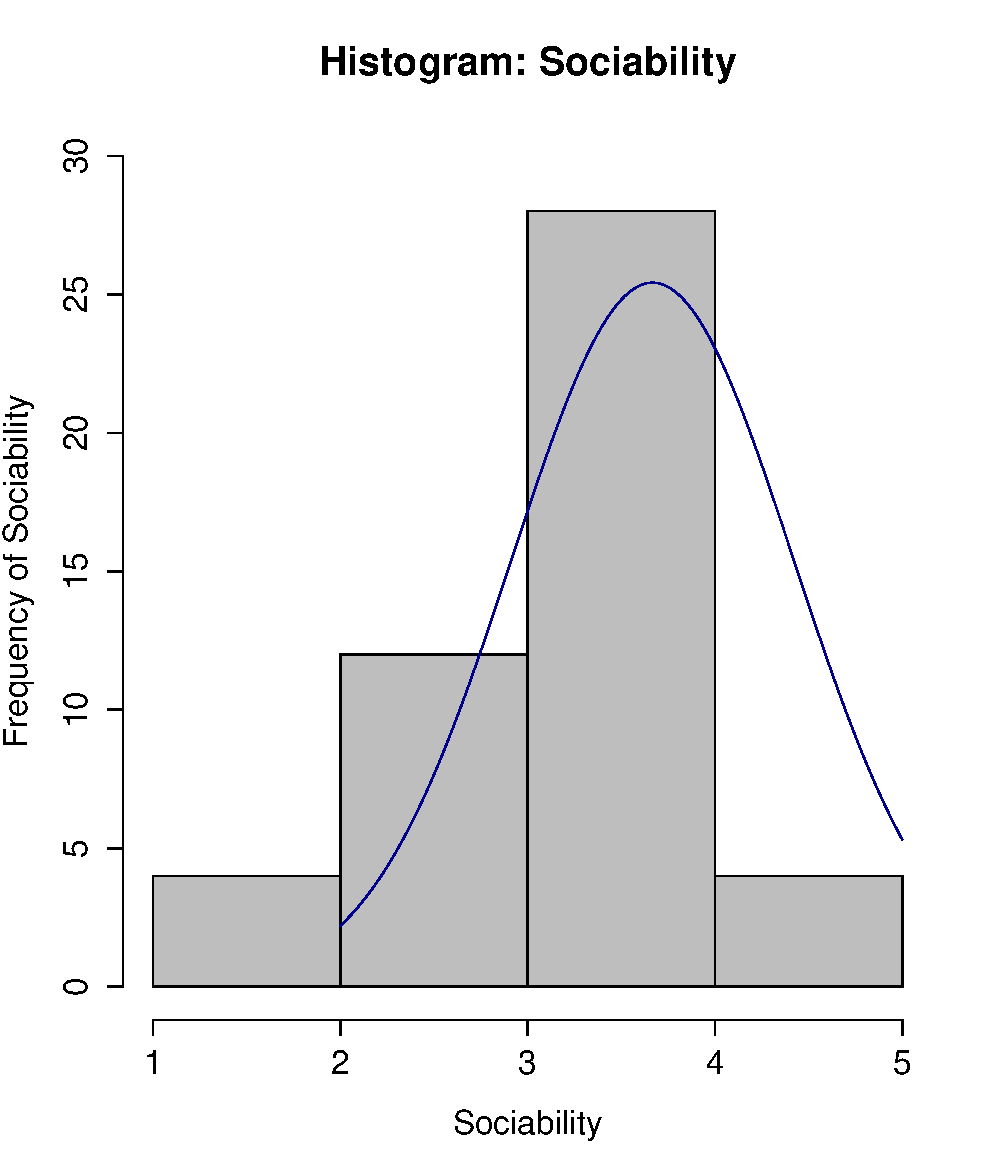
\includegraphics[scale=0.35]{./img/hist_sociability.pdf}
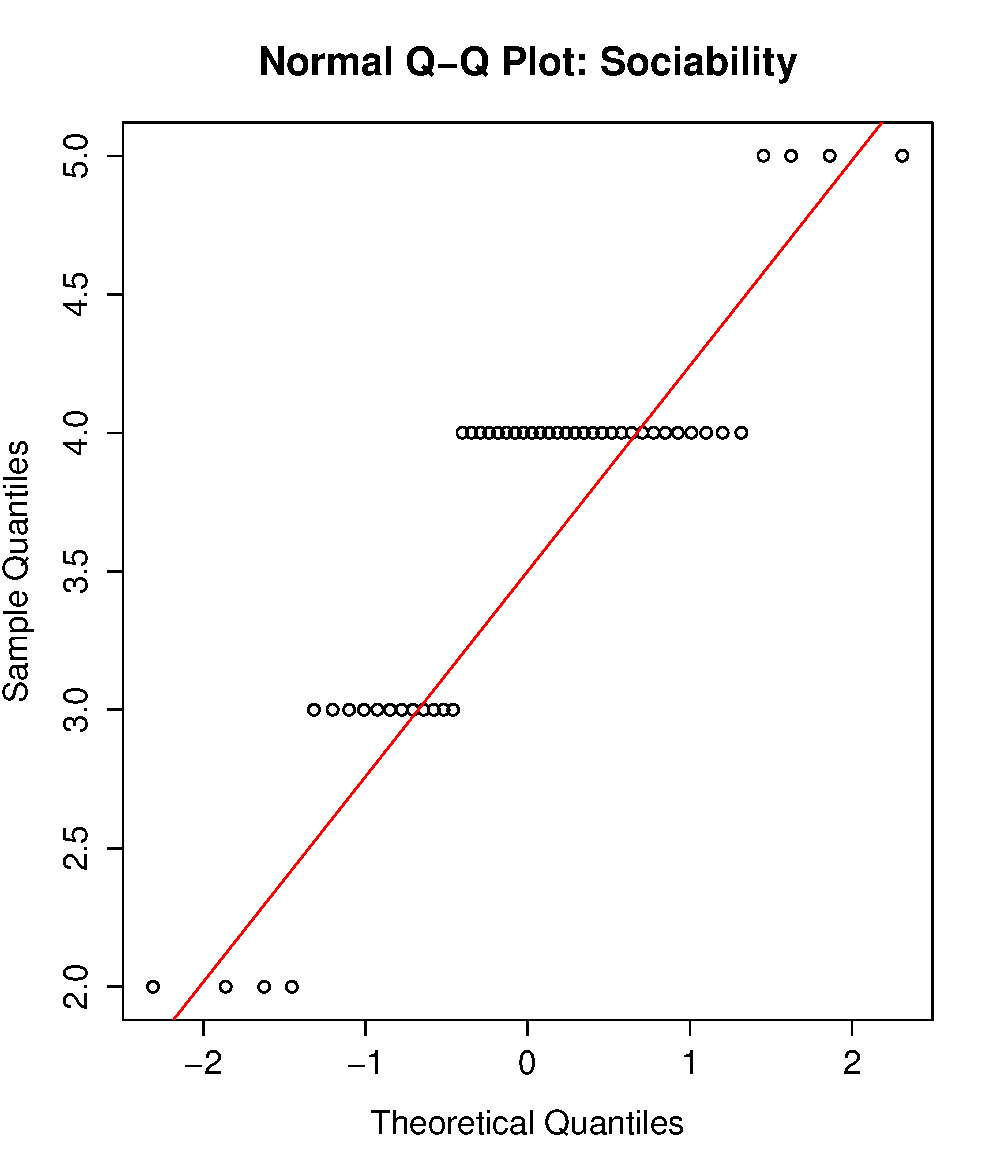
\includegraphics[scale=0.35]{./img/qqplot_sociability.pdf}
\end{figure}

\subsubsection{Facebook Hours}

Figure 5 shows the histogram and normal q-q plot for Facebook Hours. The blue curve overlay on the histogram demonstrates a non-normal distribution. The normal q-q plot also demonstrates a non-normal distribution, as the majority of data-points do not fall on the expected normal distribution line. Only non-parametric tests are applicable for this variable.

\begin{figure}[H]
\caption{Histogram and Normal Q-Q Plot: Facebook Hours}
\centering
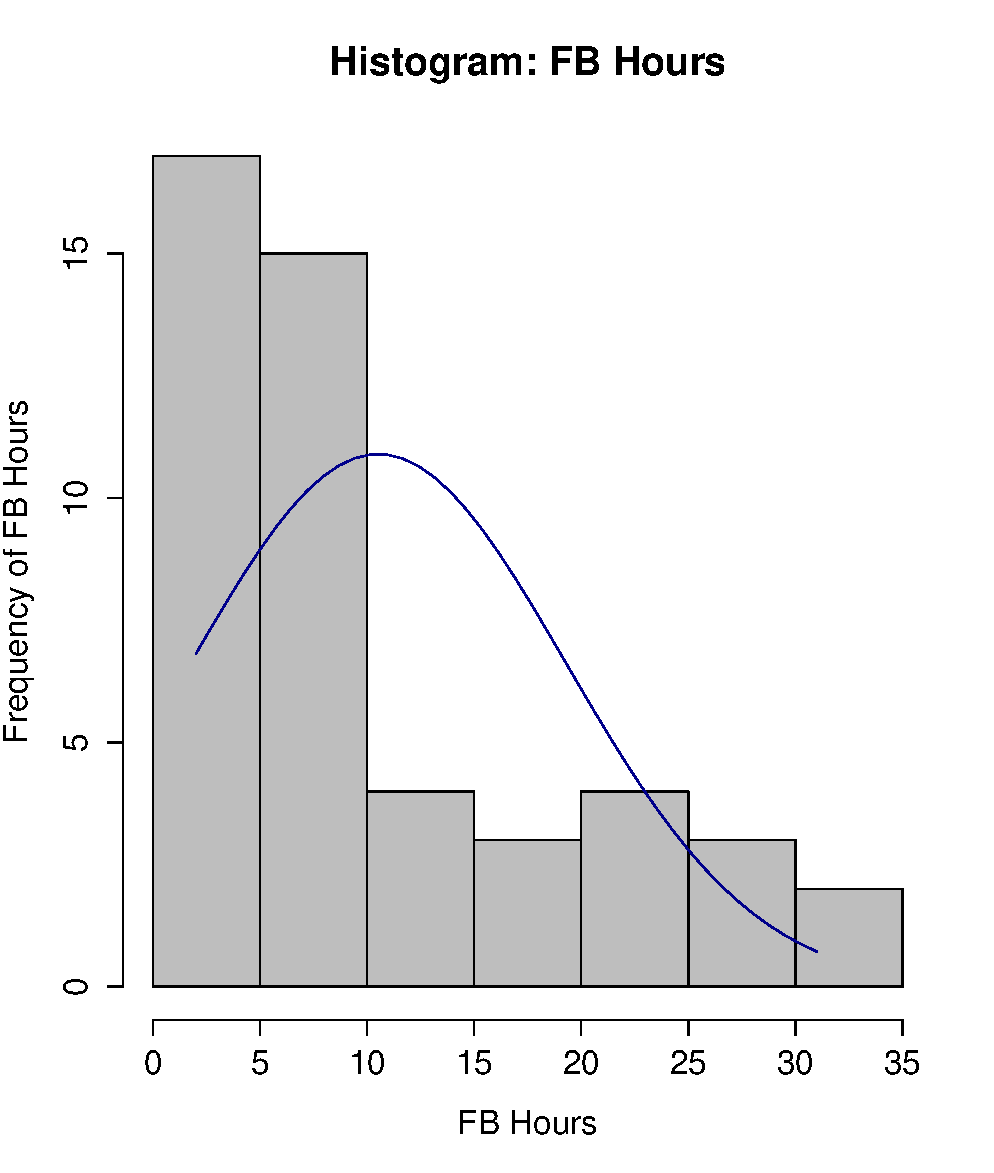
\includegraphics[scale=0.35]{./img/hist_fbhours.pdf}
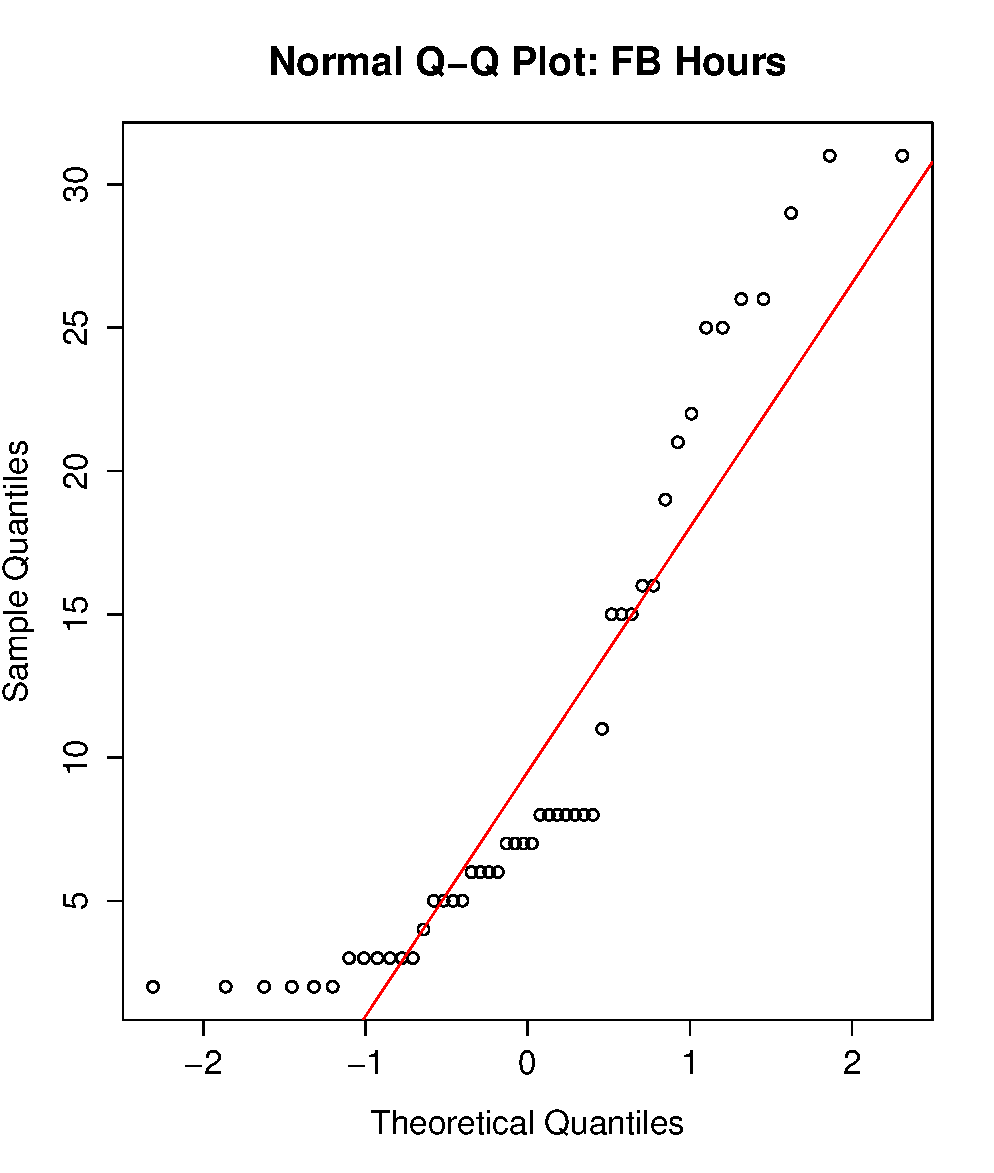
\includegraphics[scale=0.35]{./img/qqplot_fbhours.pdf}
\end{figure}

\newpage
\subsection{Bivariate inferential tests}

%\subsubsection{Pearson's correlation coefficient}

%Table 2 displays the parametric Pearson's correlation coefficient $r$ results with each variable compared with gender. Since the given data is non-normally distributed, results must be further verified by a non-parametric test. In this instance, a one-tailed test has been selected to identify a negative correlation, where 0, representing females is predicted to have higher scores than 1, which represents males, as seen in the scatter plots in Figure 6. \\
%\\
%$r$ is calculated by \citep{McKillup2011}:

%$$r = \frac{\sum_{i=1}^N (Z_{xi} \times Z_{yi})}{n - 1}$$

%$$Z = \frac{X_i - \bar{X}}{s}$$

%$$s = \sqrt{\frac{1}{N-1} \sum_{i=1}^N (x_i - \overline{x})^2}$$ **DEMO FORMULA

%The results express that gender and Facebook friends have a moderate negative correlation, gender and close friends have a weak negative correlation, and gender and Facebook hours have a moderate negative correlation. The negative correlation indicates that at $x$ variable 0, which represents women, the scores are higher than those at $x$ variable 1, which represents men. The 0 $r$ value for gender and Sociability demonstrates that there is no correlation between these two variables. These results are further illustrated in the scatter plots at Figure 6, which exhibits a reversed slope regression line for the variables with a negative correlation to gender.

%With gender as the $x$ variable, negative $r$ denotes that Facebook friends, close friends and Facebook hours increase in a reverse slope towards 0, which represents women, and conversely decreases towards 1, which represents men. The 0 $r$ value for Sociability indicates that there is no relationship between gender and sociability. These results are also illustrated in the scatter plots from Figure 6 which show the calculated regression line.

%\begin{table}[H]
%\centering
%\caption{Pearson's correlation coefficient - Gender}
%\begin{tabular}{l|l|l}
%Variable      & $r$         & p-value \\ \hline
%FB Friends    & -0.3176993  & 0.01389 \\ \hline
%Close Friends & -0.07652931 & 0.3026  \\ \hline
%Sociability   & 0           & 0.5     \\ \hline
%FB Hours      & -0.2815223  & 0.02629 \\ \hline
%\end{tabular}
%\end{table}

%Hypothetically, if there were an equal to almost equal ratio between men and women in the dataset, and all variables were of normal distribution, a fair conclusion of these results would be that there is a moderate negative correlation between gender and the number of Facebook friends and hours spent on Facebook. In other words, the negative correlation indicates that females have a greater network size than men, and spend more time on Facebook than men. With significant p-values $< \alpha = 0.05$, the null hypothesis that there are no correlations between gender and network size or gender and hours would be rejected. 

%While Close friends exhibits a negative correlation, the calculated p-value is insignificant, being $> \alpha = 0.05$. Therefore the null hypothesis that there are no correlations between gender and Close friends survives. Sociability's 0 $r$ value indicates there are no correlations at all.

%However, the data is non-normally distributed and the results must be further verified by non-parametric tests. Additionally, three points of bias are introduced while testing the correlation between gender and the selected variables. The decision to include an identified outlier has created bias towards higher scores for female Facebook friends. And while males and females both have a maximum score of 31 for Facebook hours, the small number of female participants has increased the female Facebook hours mean higher than that of men. In spite of females having a much lower Close friends maximum score than men, the small number of female participants has lead to an increased female Close friends mean. Therefore, there is not enough evidence within the dataset to provide any conclusions.

%However, since there is such a small representation of women in the sample set, there is insufficient evidence to provide a conclusion. Additionally, Pearson's method only applies to normally distributed variables and the variables measured are non-normally distributed. Therefore, the results must be further verified by non-parametric tests.

\subsubsection{Scatter plots and regression}

Figure 6 displays scatter plots with a linear regression overlay in comparison with Gender and Facebook Friends, Close Friends, Sociability and Facebook Hours.

The results indicate a moderate negative relationship between Gender and Facebook Friends, and between Gender and Facebook Hours. A weak negative relationship is observed between Gender and Close Friends, and no relationship at all between Gender and Sociability.

In other words, the negative relationships exhibit that women, represented as 0 on the $x$ axis, tend to have higher scores than men, shown as 1 on the $x$ axis, in Facebook Friends, Close Friends and Facebook Hours, as the regression line illustrates a reversed slope from 0 to 1.

However, linear regression analysis assumes that data is normally distributed and therefore is not a suitable test with the current dataset \citep[p. 263]{McKillup2011}. Linear regression is calculated with the following formulas \citep[p. 247-249]{McKillup2011}.\\
\linebreak

To calculate the average slope of the regression line:
 
$$b = \frac{\sum_{i=1}^N(X_i - \bar{X})(Y_i - \bar{Y})}{\sum_{i=1}^N(X_i - \bar{X})(X_i - \bar{X})}$$ \linebreak

To calculate the intercept at the $y$ axis:

$$a = \bar{Y} - b\bar{X}$$ \linebreak

Due to the reliance of the sample mean in linear regression analysis, the result for Facebook Friends has been influenced by the inclusion of a previously identified outlier score from a female participant. And while men and women both have a maximum score of 31 for Facebook Hours, the small number of female participants allowed the female Facebook Hours mean to increase higher than that of men. In spite of women having a much lower Close Friends maximum score than men, the small number of female participants also lead to an increased female Close Friends mean. Therefore, it is apparent that linear regression is not a suitable test, and there is simply not enough data from female participants to provide any conclusions.

\begin{figure}[H]
\caption{Scatter Plots}
\centering
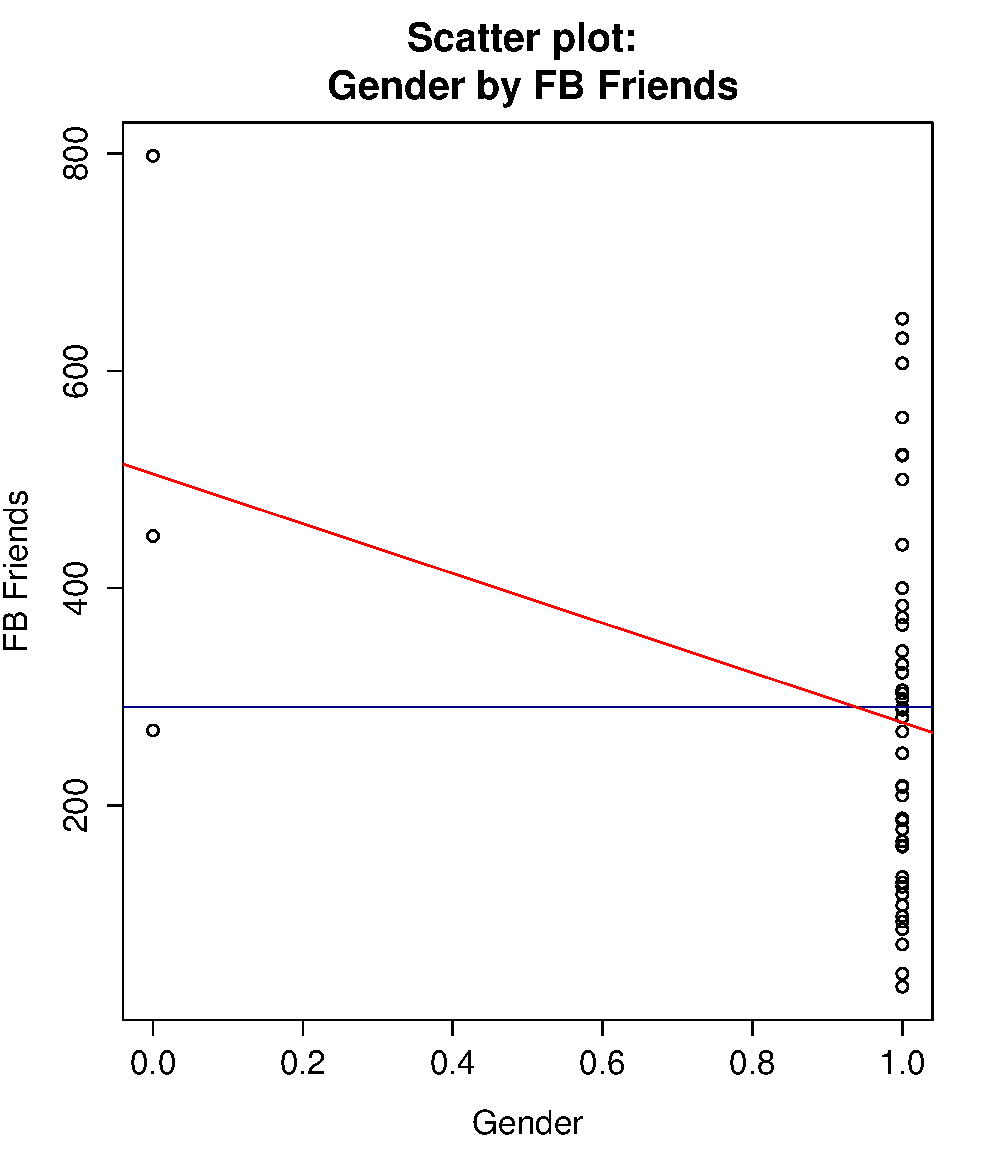
\includegraphics[scale=0.44]{./img/scatplot_fbfriends.pdf}
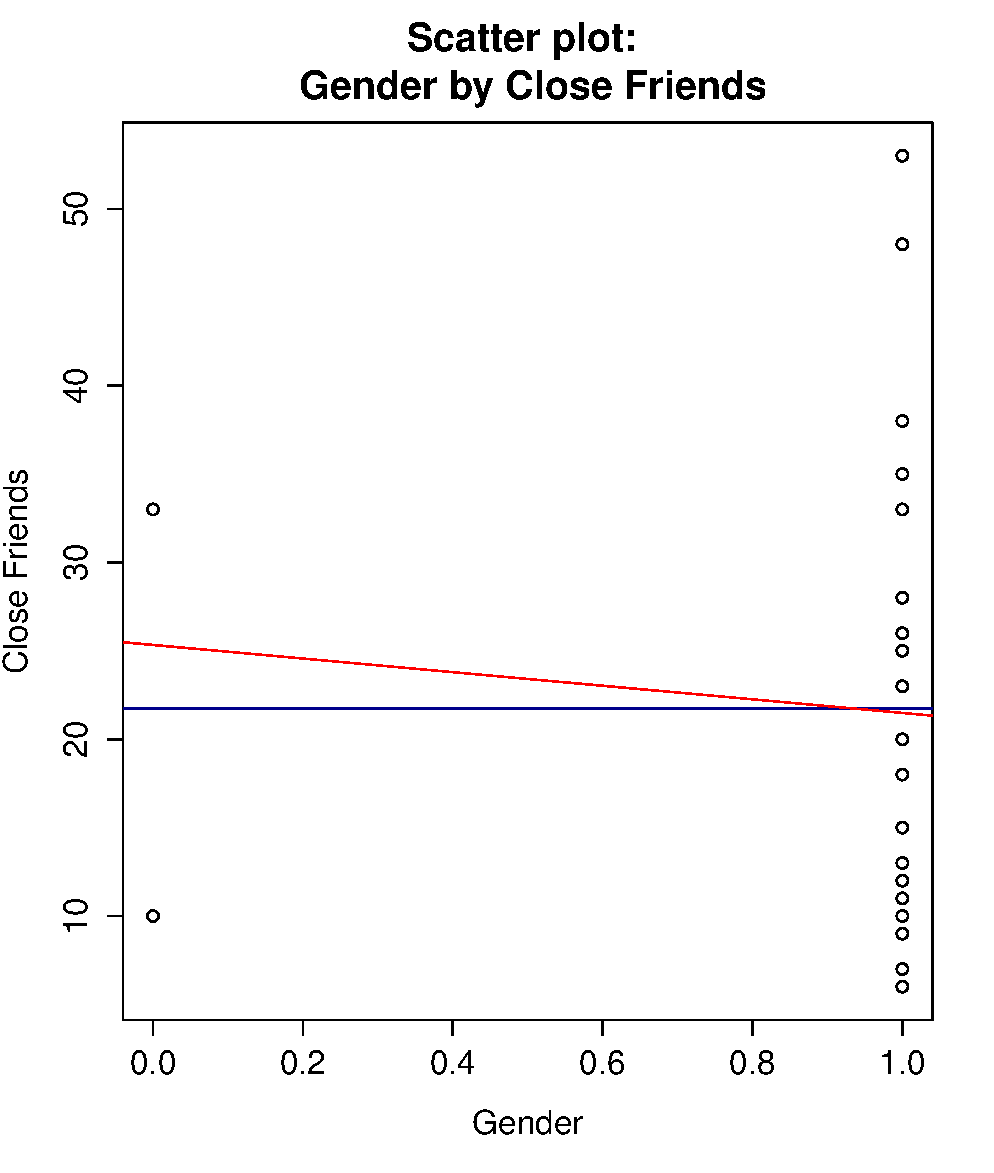
\includegraphics[scale=0.44]{./img/scatplot_closefriends.pdf}
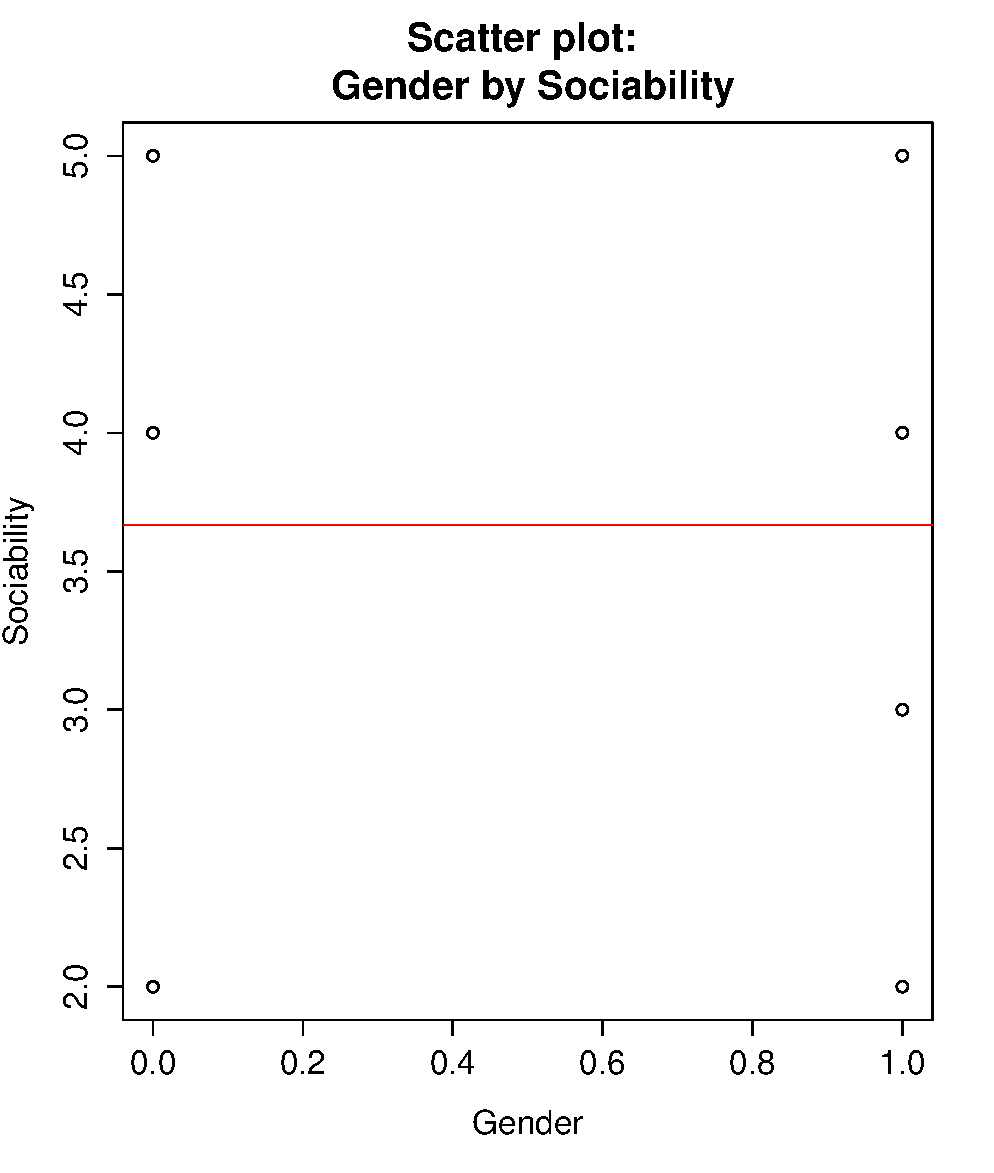
\includegraphics[scale=0.44]{./img/scatplot_sociability.pdf}
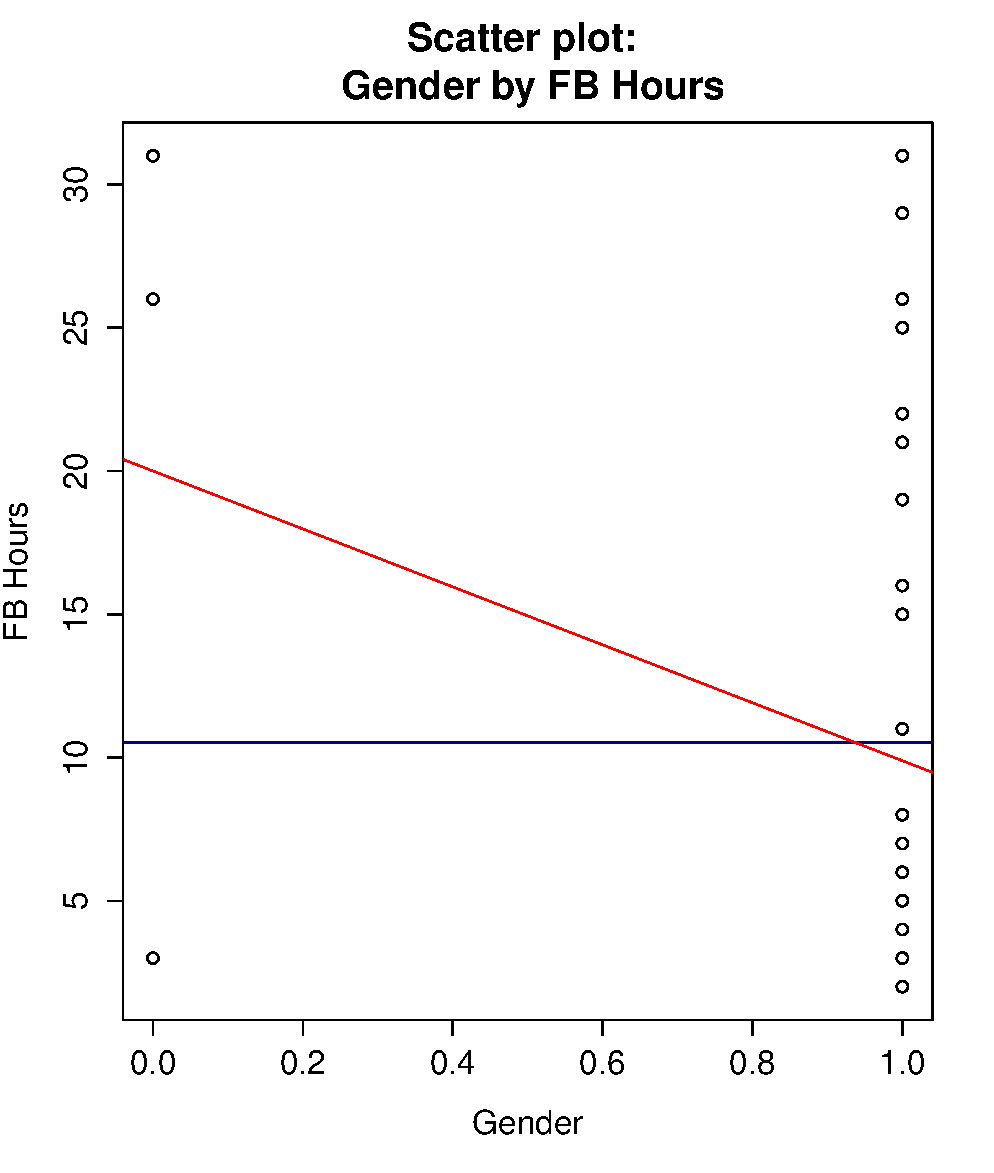
\includegraphics[scale=0.44]{./img/scatplot_fbhours.pdf}
\end{figure}

\subsubsection{Spearman's correlation coefficient}

A non-parametric correlation test has been selected to identify any correlation between Gender and Facebook Friends, Close Friends, Sociability or Facebook Hours. Table 3 displays the non-parametric Spearman's correlation coefficient results for each variable compared with Gender. A one-tailed test has been chosen due to the expectation that women will have higher scores than men, as seen in Figure 6. 

$r_s$ is calculated by ranking the scores, then calculating the correlation coefficient using the following formula \citep[p. 359]{Gauthier2001}, where $d$ = the difference between each pair of ranks from the values of variables $x$ and $y$, and $n$ = the number of paired values in the sample:

$$r_s = 1 - \frac{6\sum_{i=1}^Nd_i^2}{n(n^2-1)}$$\linebreak

A moderate negative correlation has been found between Gender and Facebook Friends ($r_s = -0.2391, N = 48, P > 0.05$), and a moderate negative correlation has been found between Gender and Facebook Hours ($r_s = -0.1747, N = 48, P > 0.05$). However, p-values for all tests are considered insignificant  being $> \alpha = 0.05$. Therefore, the null hypothesis that there are no correlations between Gender and the selected variables is not rejected.

%Similar correlation results are found from those in the previous parametric test. However, in this instance, a weak negative correlation is also found between gender and Sociability. Furthermore, all p-values in this test are considered insignificant being $> \alpha = 0.05, N = 48$. Therefore, the null hypotheses that there are no correlations between gender and the selected variables is not rejected. 

%Facebook friends exhibits the most significant p-value where H$_0$ could potentially be rejected.

Two-tail and negated one-tail tests were also performed, only to find higher, insignificant p-values.

\begin{table}[H]
\centering
\caption{Spearman's correlation coefficient - Gender}
\begin{tabular}{l|l|l}
Variable      & $r_s$      & p-value \\ \hline
FB Friends    & -0.2391999  & 0.05077 \\ \hline
Close Friends & -0.08123761 & 0.2915  \\ \hline
Sociability   & -0.04207032 & 0.3882  \\ \hline
FB Hours      & -0.1747336  & 0.1174  \\ \hline
\end{tabular}
\end{table}

Since all variables being tested are non-normally distributed, Spearman's non-parametric method is a suitable test and results considered reliable. However, the insignificant p-values indicate that the higher scores for women have occurred by chance due to the fact that there are so few female observations in the sample.

%However, three points of bias are introduced while testing the correlation between gender and the selected variables. The decision to include an identified outlier has created bias towards higher scores for female Facebook friends. And while males and females both have a maximum score of 31 for Facebook hours, the lack of gender balance has raised the female mean for Facebook hours, thus creating a bias towards higher Facebook hours for females. In fact, females have a much lower Close friends maximum score than men, however, due to the small number of female participants, the mean for that variable is higher than that of men. Therefore, there is not enough evidence within the datasete to provide any conclusions.
%The same could also be said for Close friends. Therefore, the issue still applies, that women are under represented in this study, and there is not enough evidence within the dataset to provide any conclusions.

%Again, if the dataset included a balanced ratio between men and women, Facebook friends $\rho$ could be interpreted to support the thesis statement ``Gender is related to the size of a user's Facebook network'', demonstrating that in general, women have more Facebook friends than men. Facebook hours $\rho$ could also be interpreted to support the thesis statement ``Gender is related to the amount of time a user spends on Facebook'', illustrating that in general, women report higher hours of Facebook use than men.

\subsubsection{Wilcox rank sum test}

%wilcox.test(FB_friends ~ Gender, alt="g", conf.int=T) R-code

A non-parametric independent samples test has been selected to test the null hypothesis that the distribution of scores of the selected variables between men and women are equal \citep{Coolican2014}. A one-tail test has been chosen due to the expectation that women will have higher scores than men, as seen in Figure 6. The results of this test are shown in Table 4. 

\begin{table}[H]
\centering
\caption{Wilcox rank sum test - Gender}
\begin{tabular}{l|l|l}
Variable      & W    & p-value \\ \hline
FB Friends    & 106  & 0.05277 \\ \hline
Close Friends & 80.5 & 0.2961  \\ \hline
Sociability   & 73.5 & 0.3957  \\ \hline
FB Hours      & 95.5 & 0.1197  \\ \hline
\end{tabular}
\end{table}

Similar insignificant p-values $> \alpha = 0.05$ are found to those of the Spearman's correlation coefficient test, seen in Table 3. While it is possible to conclude that the null hypothesis survives, there is not enough female observations in the dataset to provide conclusive evidence that these test results are accurate.